\section{命名空间}
C++为我们提供了丰富的函数、类和对象,我们只需要若干 \lstinline@#include@ 指令就可以把我们需要的功能收入囊中。这很方便,但也可能导致一些问题。笔者有一次在调尝试调用自己写的 \lstinline@swap@ 函数:
\begin{lstlisting}
void swap(int &a, double &b) {
    int tmp {a};
    a = b;
    b = tmp;
}
int main() {
    int a {3};
    double b {5};
    swap(a, b);
    cout << a << ' ' << b; //预期输出5 3
}
\end{lstlisting}
这段代码的调试结果合乎预期,而当我把 \lstinline@double b{5}@ 改成 \lstinline@int b{5}@ 的时候,却也输出了同样的内容。\par
但是不应该啊,按理说 \lstinline@int@ 类型的 \lstinline@b@ 会转换成 \lstinline@double@ 类型的临时变量,但这个临时变量是右值\footnote{我们将在精讲篇谈左值/右值的问题。},不可能被 \lstinline@swap@ 接收。为什么这个函数仍然正常运行并且给出了``正确''的输出呢?\par
再深入研究之后我才发现,原来程序很本就没有调用我自定义的 \lstinline@swap@ 函数,它调用的是标准库自带的 \lstinline@swap@!
\begin{lstlisting}
template< class T >
void swap( T& a, T& b ) noexcept( /* ... */ );
\end{lstlisting}
也就是从这个时期起,我逐渐放弃了使用 \lstinline@using namespace std@ 和 \lstinline@#include<bits/stdc++.h>@\footnote{\lstinline@bits/stdc++.h@ 是GCC编译器中允许的一个不标准的头文件。使用这个头文件可以让我们一次性包含许多常见头文件。这种用法被普遍认为是``不好的习惯'',详见\href{https://stackoverflow.com/questions/31816095/why-should-i-not-include-bits-stdc-h}{Why should I not \#include <bits/stdc++.h>? - Stack Overflow}。}这两个习惯。\par
几乎所有初学者都会无一例外地认为 \lstinline@using namespace std@ 是很方便的;而通篇累牍的 \lstinline@std::cin@ 和 \lstinline@std::cout@ 则显得十分麻烦。但是当我们的代码量非常大之后,我们难免会起一些与标准库中名字相冲突的变量、函数、枚举、结构和类。举几个例子吧:
\begin{itemize}
    \item \lstinline@list@, \lstinline@map@, \lstinline@array@, \lstinline@queue@, \lstinline@set@, \lstinline@string@, \lstinline@pair@;
    \item \lstinline@copy@, \lstinline@find@, \lstinline@move@, \lstinline@search@, \lstinline@count@, \lstinline@sample@;
    \item \lstinline@next@, \lstinline@begin@, \lstinline@end@, \lstinline@data@, \lstinline@size@;
    \item \lstinline@function@, \lstinline@future@, \lstinline@thread@, \lstinline@yield@;
    \item \ldots\ldots
\end{itemize}
以上这些,有些是类模板,有些是函数模板,或者还有别的。这些名字你可能未必都知道,但是总会有些单词是你熟悉的吧!一旦我们不慎使用了这些名字,那么要么程序报错,你找了半天才知道问题所在;要么程序不报错,但至于究竟使用了哪个名字,做了什么,就不敢保证了。\par
试想,当你在用这些名字定义函数的时候,你是在重载它们;而当你在用这些名字定义类的时候,你会被编译器禁止(因为类不能重载)。被编译器禁止还是更好的选择,因为它在编译期就能帮你检查出错误来;但如果把这些错误留到运行期,那就很难说会发生什么了!\par
解决这个问题的方法很多样。我们可以自己有意识地避开这些名字(一般来说,只要你经验丰富,就不太容易在这个问题上翻车);或者干脆点,不用 \lstinline@using namespace std@ 了\footnote{不过我并不建议读者彻底杜绝 \lstinline@using namespace std@ 的使用。这种语法并不像 \lstinline@bits/stdc++.h@ 库或 \lstinline@goto@ 语句那样饱受诟病,仍然是许多程序员图省事的最佳选择。}。那么究竟什么是 \lstinline@namespace@,我们为什么要用它,又怎么用它呢?本节就来讲解这些问题。\par
\subsection*{什么是命名空间?}
想象一下Windows电脑的文件资源管理器——就以D盘为例吧。我们可以直接把文件存放在D盘的主目录下,不过我们很少这么做;我们绝大多数时候是在D盘中建立一些文件夹,甚至是文件夹套文件夹,然后把具体的文件存放到这些文件夹中。简化起见,我们只在D盘中用两个文件夹。这两个文件夹中各有一份名叫\texttt{Test.txt}的文本文档\footnote{它们二者之间不是快捷方式的关系,是真正意义上独立的文件。否则这个讨论就没什么意义了。}。它们虽然同名,但它们不冲突,因为它们在不同的文件夹下。修改其中一个\texttt{Test.txt}中的内容也不会对另一个\texttt{Test.txt}造成什么影响。\par
那么我们是不是可以这样认为:这两个文件虽然重名,但它们存在于不同的空间中,所以不会有什么冲突。如果我们想访问这两个文件,我们也肯定会通过不同路径来找。这样,一切可能的冲突都解决了。\par
\begin{figure}[htbp]
    \centering
    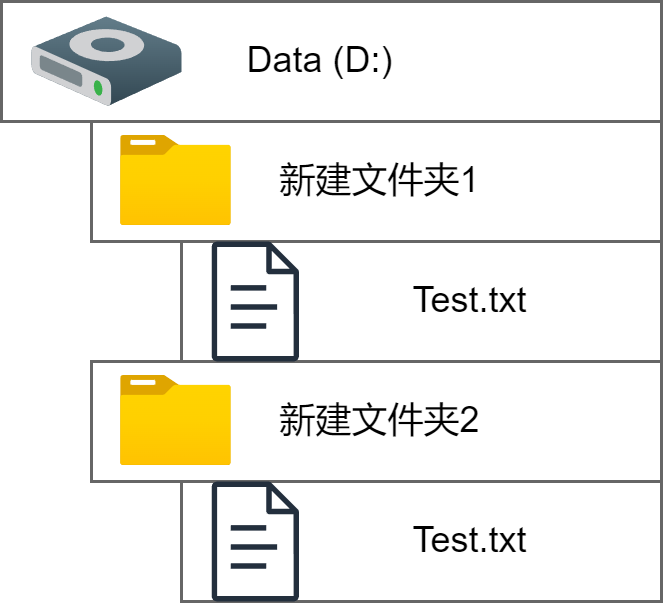
\includegraphics[width=0.5\textwidth]{../images/generalized_parts/07_file_explorer_and_namespaces.png}
    \caption{Windows文件资源管理器中的重名文件}
\end{figure}
命名空间也是这样的道理。在不同的命名空间中,我们可以按我们的需要来给变量、函数和类起名字,而不必担心与其它命名空间中的什么东西重名。\par
不过,实际上的命名空间还是与Windows资源管理器的结构不同的。接下来我们讲解一些有关命名空间的最基本规则。\par
\subsection*{命名空间的定义和使用}
在所有作用域之外,也就是在函数、类、枚举等内容之外,有一个\textbf{全局命名空间(Global namespace)}。在全局命名空间中定义的名字,在其它任何地方都可以使用\footnote{具体说来,指的是此源代码中,从该名称声明处开始的位置。头文件中定义的内容看似在整个源文件中可用,那只是因为我们把文件包含写在源文件开头所致。}。比如说,我们声明的那些函数,就在整个翻译单元的所有位置中可用。\par
\begin{lstlisting}
struct A {
    //...
}; //该类定义在全局命名空间中,对后文全局可见
void fun(); //该函数声明在全局命名空间中,对后文全局可见
constexpr double Pi {3.14}; //该常量表达式定义在全局命名空间中,对后文全局可见
extern unsigned count; //该变量声明在全局命名空间中,对后文全局可见
int main() {
    //这里可以使用A, fun, Pi, count等名字,没有任何问题
}
\end{lstlisting}\par
我们可以使用 \lstinline@namespace@ 关键字来自定义命名空间。C++中使用了 \lstinline@std@ 命名空间,我们所熟知的 \lstinline@cin@, \lstinline@cout@ 和 \lstinline@endl@ 等等,就在 \lstinline@std@ 命名空间中。\par
为了使用 \lstinline@std@ 命名空间中的名字,我们可以通过作用域解析运算符\footnote{有些资料会把它叫作``操作符''而不是``运算符'',因为作用域解析更像是一种操作而非运算,其实它们在英文中都叫Operator,这里可以区分也可以不区分。} \lstinline@::@(两个紧密排列的冒号,这是``一个''运算符,不可以分开写)。比如说要用 \lstinline@std@ 命名空间中的 \lstinline@cin@ 对象,我们就可以写成 \lstinline@std::cin@。
\begin{lstlisting}
int main() {
    int number;
    std::cin >> number; //使用std命名空间中的cin对象
}
\end{lstlisting}\par
我自己写代码时常常用自定义的 \lstinline@cppHusky@ 命名空间,并把我想要写的函数定义在其中。
\begin{lstlisting}
namespace cppHusky {
    template<typename T>
    T max(T a, T b) {
        return a > b ? a : b;
    } //定义函数模板max
    template<typename T>
    T min(T a, T b) {
        return a < b ? a : b;
    } //定义函数模板min
}; //注意分号结尾
\end{lstlisting}
在 \lstinline@cppHusky@ 命名空间中定义的 \lstinline@max@ 就不同于 \lstinline@algorithm@ 库中,在 \lstinline@std@ 命名空间中定义的 \lstinline@max@。
\begin{lstlisting}
    std::cout << std::max(3, 5) << std::endl; //注意endl也在std命名空间中
    std::cout << cppHusky::max(3, 5) << std::endl;
\end{lstlisting}
这里我们使用的两个 \lstinline@max@ 函数分别位于两个命名空间中,互不冲突。\par
命名空间之间还可以嵌套定义,比如 \lstinline@std@ 命名空间中还嵌套定义了 \lstinline@ios_base@ 命名空间,它们二者的大致关系是
\begin{lstlisting}
namespace std { //命名空间std
    //...
    namespace ios_base { //std中的命名空间ios_base
        //...
    };
};
\end{lstlisting}\par
在 \lstinline@ios_base@ 命名空间中有一些 \lstinline@fmtflags@ 常量表达式,比如 \lstinline@boolalpha@\footnote{我们曾讲过,\lstinline@std::cout@ 在输出 \lstinline@bool@ 型数据时默认按整数形式输出。如果我们要按布尔型数据输出,可以用 \lstinline@cout.setf(ios_base::boolalpha)@,详见2.2节。}。如何获取到它呢?首先它在 \lstinline@ios_base@ 命名空间中,所以我们要使用 \lstinline@ios_base::boolalpha@。而倘若我们没有直接 \lstinline@using@ 这个 \lstinline@std@ 命名空间,我们还需要通过 \lstinline@std@ 才能访问到 \lstinline@ios_base@ 命名空间,所以我们要写成 \lstinline@std::ios_base::boolalpha@ 才行。\par
\begin{lstlisting}
    bool judgement {2>3};
    std::cout.setf(std::ios_base::boolalpha); //设置成按布尔型输出
    std::cout << judgement; //将输出false
\end{lstlisting}\par
如果我们需要使用全局命名空间中的名字 \lstinline@x@,我们可以直接写成 \lstinline@::x@ 的形式。
\begin{lstlisting}
int x {3}; //在全局命名空间中
int main() {
    int x {5}; //不在全局部名空间中
    std::cout << x << std::endl; //将输出5
    std::cout << ::x << std::endl; //将输出3
}
\end{lstlisting}
这里我们定义了两个 \lstinline@x@,读者可能会感到困惑。不要担心,我们会在下一节中介绍它。\par
\lstinline@namespace@ 块有一个特点,它是可以扩展的。
\begin{lstlisting}
//以下是Header.hpp
namespace cppHusky {
extern std::stringstream cin; //声明,其中的stringstream需要sstream库
template<typename T>
constexpr const char* Tname(const T &object)noexcept{
    return typeid(object).name();
}
template<typename T>
constexpr const char* Tname()noexcept{
    return typeid(T).name();
}
};
//以下是main.cpp
#include "Header.hpp"
int main() {/*...*/}
namespace cppHusky {
std::stringstream cin {"1024"}; //定义
};
\end{lstlisting}
我自己写代码的时候,常常会用这里的 \lstinline@cppHusky::cin@ 和 \lstinline@cppHusky::Tname@ 来进行测试。读者尚且不需要知道它们是用来干什么的,只需要关注整个代码的结构就可以了。\par
我们曾介绍过文件包含的机制。在源文件中,\lstinline@#include"Header.hpp"@ 指令会被预处理器替换成\texttt{Header.hpp}中的内容,所以我们可以认为,头文件中的指令被复制到了源文件中。那么在这里,就出现了两个命名空间的定义:
\begin{lstlisting}
//等效于以下写法:
namespace cppHusky {
//在这里声明了cin并定义了Tname
};
namespace cppHusky {
//在这里定义cin
};
\end{lstlisting}
在第一次使用 \lstinline@namespace cppHusky@ 的时候,我们是在定义一个新的命名空间;而在第二次使用 \lstinline@namespace cppHusky@ 的时候,因为 \lstinline@cppHusky@ 已经定义,所以这里新增的内容只是对 \lstinline@cppHusky@ 命名空间的内容扩充。在这两段代码编译完毕之后,\lstinline@cppHusky@ 命名空间中就既有了 \lstinline@Tname@ 的定义,又有了 \lstinline@cin@ 的定义。我们还可以在其它地方继续通过 \lstinline@namespace cppHusky@ 添加新的内容。\par
之所以允许这样做,是因为我们会有``把不同头文件/源文件中定义的名字放在同一空间下''的需求。比如对于 \lstinline@std@ 命名空间来说,C++在 \lstinline@iostream@ 头文件中定义了 \lstinline@std::cin@,在 \lstinline@cstring@ 头文件中定义了 \lstinline@std::strlen@,在 \lstinline@algorithm@ 头文件中定义了 \lstinline@std::max@ 和 \lstinline@std::min@,诸如此类……它们处于不同文件中,但只要用 \lstinline@namespace std@ 就可以把它们一同加到这个空间中来,这岂不是很方便?\par
\subsection*{\lstinline@using@ 声明}
如果每次都要靠作用域解析运算符 \lstinline@::@ 来访问非全局变量,那就显得太麻烦了。所以初学者一般很喜欢这样写,一劳永逸:
\begin{lstlisting}
using namespace std;
\end{lstlisting}
这个语句的作用是,把 \lstinline@std@ 整个命名空间引入到此处。于是 \lstinline@std@ 命名空间中的所有类、函数和对象都在此空间中可用。如果我们把 \lstinline@using namespace@ 写在全局作用域中(我们一般这么做),那么这个命名空间中的内容就被引入到全局作用域中。
\begin{lstlisting}
using namespace std; //把 \lstinline@std@ 命名空间中的内容引入全局作用域
int main() {
    int num[3];
    std::cin >> num[0]; //标准写法
    ::cin >> num[1]; //既然引入了全局作用域,那cin就是全局作用域的一部分了
    cin >> num[2]; //会进行名称查找,进而找到全局作用域中的cin,详见下一节
}
\end{lstlisting}
当然,我们在上文中已经提到过,\lstinline@using namespace std@ 会把 \lstinline@std@ 中的所有内容都引入全局作用域,而其中恰好有些是容易重名的。\par
所以我们还可以有选择地指定把个别常用的名字引入全局作用域。这里也需要用到 \lstinline@using@ 语法。
\begin{lstlisting}
using std::cin, std::cout, std::endl;
\end{lstlisting}
这样我们就可以有选择地把这三个常用且不易重名的对象引入到全局作用域,以后直接用它们即可。\par
关于要不要用 \lstinline@using@ 来引入命名空间,以及怎么引入的问题,不同的人有不同的见解。大致说来,如果你要追求严谨、准确、无歧义的代码,那么你就要忍受使用诸如 \lstinline@std::@ 这种写法造成的麻烦;如果你要追求简洁、方便的代码,那么你就需要有意识地防范出现名称冲突的问题——总之有利有弊。\par
